\chapter{Data}
\label{app:ch:data_insights}
In this chapter, additional information regarding the data used in this work are provided.

\textbf{OHLC Distribution} \quad It is subsequently displayed in Tab.\ \ref{tab:appendix_ohlc_reference_norm} the aggregate statistics for the z-score normalized OHLC data and their mean and standard deviation (Tab.\ \ref{tab:appendix_ohlc_zscore_params}).

\begin{table}[htbp]
\centering
\footnotesize
\renewcommand{\arraystretch}{1.28}
\setlength{\tabcolsep}{6pt}
\begin{tabular}{l r r r r}
\toprule
\textbf{Statistic} & \textbf{Close} & \textbf{High} & \textbf{Low} & \textbf{Open} \\
\midrule
Mean          &  0.0000 & 0.0000 & 0.0000 &  0.0000 \\
Std           &  1.0000 &  1.0000 &  1.0000 &  1.0000 \\
Min           & $-$44.8905 & $-$44.9547 & $-$74.1453 & $-$87.0546 \\
$q_{0.01}$    & $-$2.7247 & $-$1.4785 & $-$3.4485 & $-$2.6747 \\
$q_{0.05}$    & $-$1.4216 & $-$0.8963 & $-$1.5955 & $-$1.1570 \\
$q_{0.25}$    & $-$0.4350 & $-$0.5050 & $-$0.2970 & $-$0.2697 \\
Median        & $-$0.0216 & $-$0.1908 &  0.1894 & $-$0.0244 \\
$q_{0.75}$    &  0.4330 &  0.2699 &  0.5344 &  0.2814 \\
$q_{0.95}$    &  1.4386 &  1.5226 &  0.9590 &  1.1723 \\
$q_{0.99}$    &  2.7817 &  3.3728 &  1.6660 &  2.7358 \\
Max           & 33.1965 & 57.0824 & 39.3966 & 63.8070 \\
Skewness      & $-$0.5773 &  7.1008 & $-$4.3308 & $-$2.1116 \\
Ex.\ Kurtosis & 38.5 & 261.2 & 106.4 & 254.7 \\
\bottomrule
\end{tabular}
\caption{Full distributional statistics for the normalized OHLC log-returns reference dataset
($n=2{,}623{,}489$). Each channel is independently $z$-scored to zero mean and unit
variance prior to training.}
\label{tab:appendix_ohlc_reference_norm}
\end{table}

\begin{table}[htbp]
\centering
\footnotesize
\renewcommand{\arraystretch}{1.28}
\setlength{\tabcolsep}{6pt}
\begin{tabular}{l r r}
\toprule
\textbf{Channel} & \textbf{Mean} & \textbf{Std} \\
\midrule
Close & 0.000451 & 0.020867 \\
Open  & 0.000265 & 0.010859 \\
High  & 0.012179 & 0.019033 \\
Low   & $-$0.011306 & 0.017881 \\
\bottomrule
\end{tabular}
\caption{Per-channel mean and standard deviation used for $z$-score normalization of the
OHLC log-return channels prior to training.}
\label{tab:appendix_ohlc_zscore_params}
\end{table}

\textbf{OHLC Correlation} \quad For a more comprehensive dataset overview it is reported also the correlation matrix in Fig.\ \ref{fig:correlation_matrix_OHLC}.
\begin{figure}[h]
    \centering
    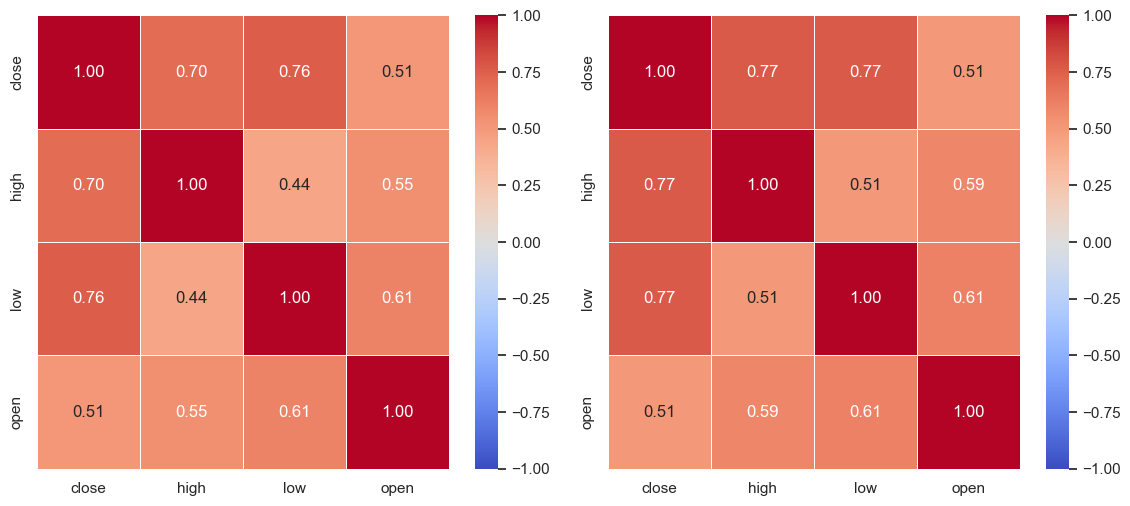
\includegraphics[width=0.7\textwidth]{images/ch4/correlation_map.png}
    \caption{Correlation Matrix for OHLC values. \emph{Left.} Correlation for concatenated data. \emph{Right.} Average correlation across files.}
    \label{fig:correlation_matrix_OHLC}
\end{figure}

\section{Decimalization}
\label{app:subsec:decimalization}
In this section it will be discussed more in depth the decimalization process briefly mentioned in  Sec.\ \ref{sec:ch4_data}, specifically what it is and how it is distributed in our training dataset.

\textbf{Introduction} \quad The decimalization process was mandated by the Securities and Exchange Commission in January 2000 and completed by the 9th of April 2001 \cite{furfine2003decimalization}. Before this period US stock prices were quoted in fractions, specifically 1/16th of a dollar, meaning that the minimum price movement needed to record an effective
change in price was 0.0625 dollars. After decimalization this changed to 1 cent.

\textbf{Characteristics} \quad 7.1928\% of all our returns are exactly 0.0. The distribution of these zero-returns is not equal, specifically they are mostly concentrated around 1980s and 1990s as it is possible to see from the Fig.\ \ref{fig:zero_returns_distribution}.

\begin{figure}[h]
    \centering
    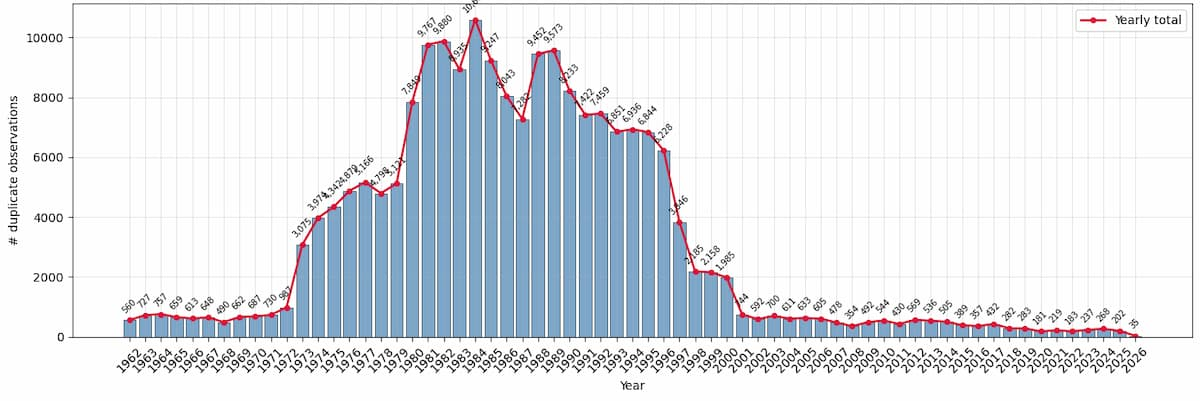
\includegraphics[width=0.7\textwidth]{images/ch4/zero_returns_distribution_cropped.jpg}
    \caption{Frequency count of absolute zero returns grouped by year.}
    \label{fig:zero_returns_distribution}
\end{figure}

The peak incidence of zero-returns occurred in 1984, with \(10{,}600\) observations, corresponding to \(21.374\%\) of that year's total returns.Interestingly, the frequency of 0\% returns drops before 1980. This is due 
to the 40-year historical minimum imposed on ticker selection (Sec.\ \ref{sec:ch4_data}): all tickers 
have data from at least April 1986, but as one moves further back in time 
the number of available observations falls considerably. Specifically, the 
number of tickers decreases from 210 with data going back to 1986, to 91 
in the 1970s, and to only 26 in the 1960s.

\textbf{Decimalization Consequences} \quad Decimalization is responsible for 
the distinctive $q_{0.02}$--$q_{0.98}$ range shape discussed in the 
experimental chapter (Ch.~\ref{ch:experiments_results}), as further 
evidenced by the evolution of the log-return distribution shown in 
Fig.~\ref{fig:log_returns_history}.


\begin{figure}[h]
\centering
\begin{subfigure}[c]{0.30\textwidth}
  \centering
  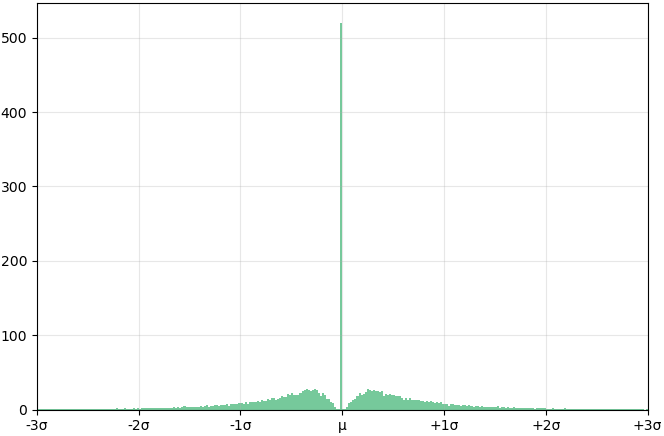
\includegraphics[width=\linewidth]{images/ch4/log_return_distribution/1970_distribution.png}
  \label{fig:grid_r1_cA}
\end{subfigure}\hfill
\begin{subfigure}[c]{0.30\textwidth}
  \centering
  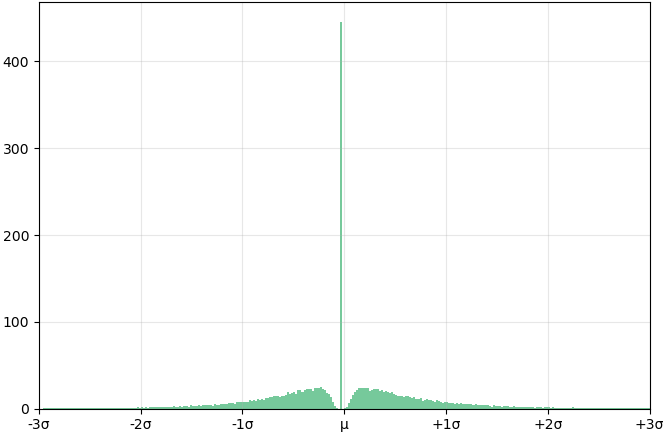
\includegraphics[width=\linewidth]{images/ch4/log_return_distribution/1980_distribution.png}
  \label{fig:grid_r1_cB}
\end{subfigure}\hfill
\begin{subfigure}[c]{0.30\textwidth}
  \centering
  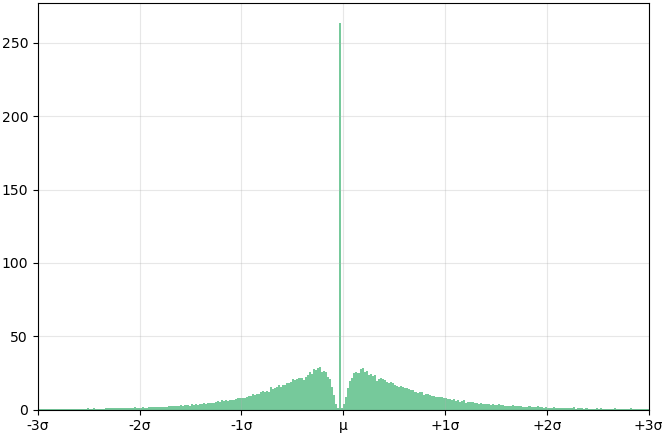
\includegraphics[width=\linewidth]{images/ch4/log_return_distribution/1990_distribution.png}
  \label{fig:grid_r1_cC}
\end{subfigure}%
\vspace{0.2em}
\begin{subfigure}[c]{0.30\textwidth}
  \centering
  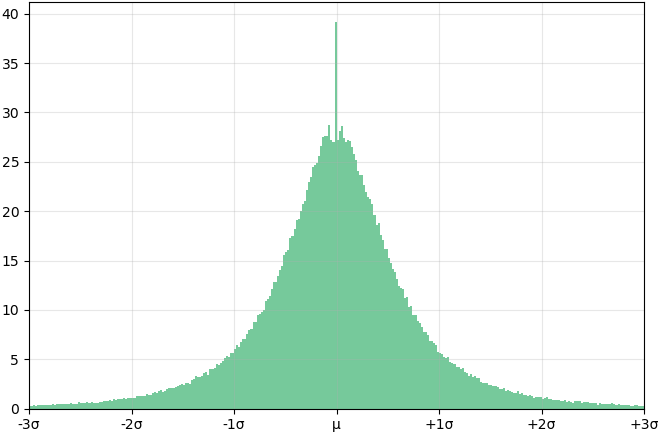
\includegraphics[width=\linewidth]{images/ch4/log_return_distribution/2000_distribution.png}
  \label{fig:grid_r2_cA}
\end{subfigure}\hfill
\begin{subfigure}[c]{0.30\textwidth}
  \centering
  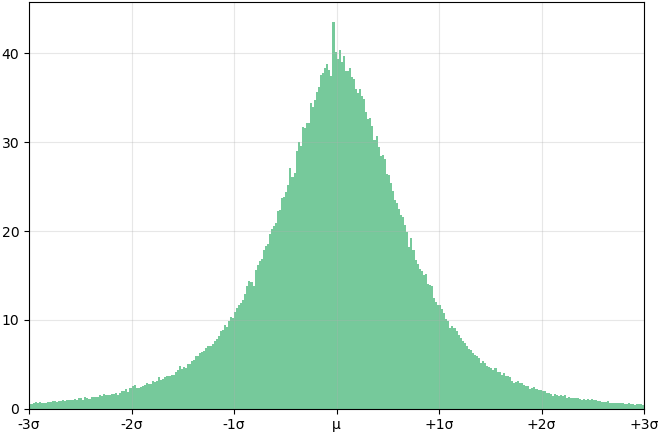
\includegraphics[width=\linewidth]{images/ch4/log_return_distribution/2010_distribution.png}
  \label{fig:grid_r2_cB}
\end{subfigure}\hfill
\begin{subfigure}[c]{0.30\textwidth}
  \centering
  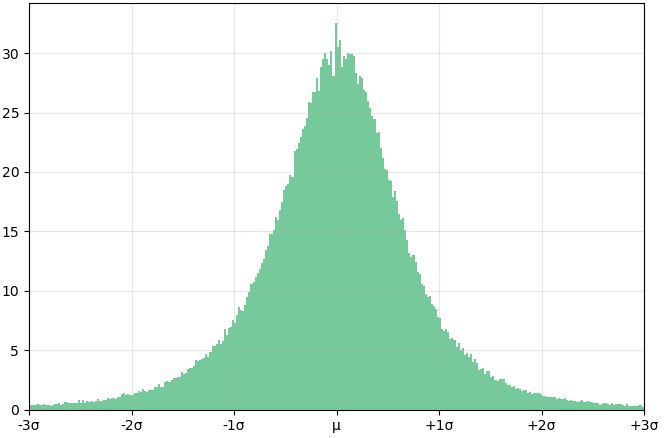
\includegraphics[width=\linewidth]{images/ch4/log_return_distribution/2020_distribution.png}
  \label{fig:grid_r2_cC}
\end{subfigure}%
\caption{Log-returns distribution by decade from 1970 (\emph{top-left}) to 2020 (\emph{bottom-right}). The decade 2020 refers to data till April 2026. Only data within the range of three standard deviations are displayed.}
\label{fig:log_returns_history}
\end{figure}